% \documentclass{standalone}

\tikzset{every node/.style={scale=1.4}}

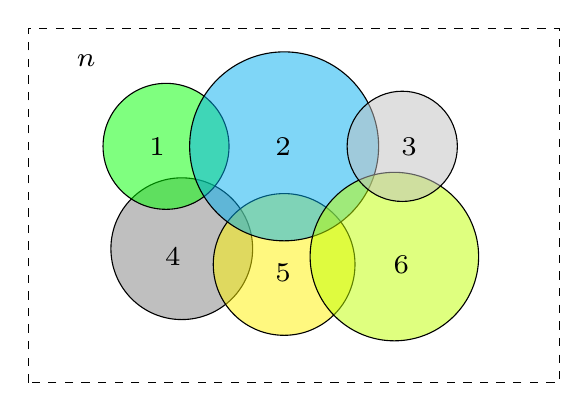
\begin{tikzpicture}
% outer dashed circle
\draw[dashed] (-0.75,1.0) rectangle (6cm, 5.5cm);

% circles 
% \draw [fill=cyan, fill opacity=0.5] (1,1) circle (1cm);
\draw [fill=gray, fill opacity=0.5] (1.2,2.7) circle (0.9cm);
\draw [fill=green, fill opacity=0.5] (1,4) circle (0.8cm);
% \draw [fill=red, fill opacity=0.5] (2.5,1) circle (1cm);
\draw [fill=yellow, fill opacity=0.5] (2.5,2.5) circle (0.9cm);
\draw [fill=cyan, fill opacity=0.5] (2.5,4) circle (1.2cm);
% \draw [fill=pink, fill opacity=0.5] (4,1) circle (1cm);
\draw [fill=lime, fill opacity=0.5] (3.9,2.6) circle (1.07cm);
\draw [fill=lightgray, fill opacity=0.5] (4,4) circle (0.7cm);


% \draw [fill=magenta, fill opacity=0.5] (1,1) circle (1cm) node {$\D_1$};
% \draw [fill=brown, fill opacity=0.5] (1,2.5) circle (1cm) node {$\D_2$};
% \draw [fill=purple, fill opacity=0.5] (2.5,1) circle (1cm) node {$\D_3$};
% \draw [fill=yellow, fill opacity=0.5] (2.5,2.5) circle (1cm) node {$\D_4$};

% labels
\node at (0.9,4) {$\D_1$};
\node at (2.5,4) {$\D_2$};
\node at (4.1,4) {$\D_3$};
\node at (1.1,2.6) {$\D_4$};
\node at (2.5,2.4) {$\D_5$};
\node at (4,2.5) {$\D_6$};
\draw (0, 5) node {$\Y^n$};

\end{tikzpicture}
